\documentclass[12pt,onecolumn]{article}

\usepackage{listings}
\usepackage{float}
\usepackage{mathtools}
\usepackage[russian]{babel}
\everymath{\displaystyle}
\usepackage{multicol}
\usepackage{blindtext}
\usepackage{amsmath} 
\usepackage{tabularray}
\usepackage[usenames]{color}
\usepackage{colortbl}
\usepackage{pbox}
\usepackage{geometry}
\usepackage{minted}
\usepackage{pgfplots}
\pgfplotsset{width=10cm,compat=1.9}

% We will externalize the figures
\usepgfplotslibrary{external}

\geometry{
  a4paper,
  top=15mm, 
  right=10mm, 
  bottom=15mm, 
  left=10mm
}

\definecolor{dkgreen}{rgb}{0,0.6,0}
\definecolor{gray}{rgb}{0.5,0.5,0.5}
\definecolor{mauve}{rgb}{0.58,0,0.82}

\lstset{frame=tb,
  language=sh,
    aboveskip=3mm,
      belowskip=3mm,
        showstringspaces=false,
	  columns=flexible,
	    basicstyle={\small\ttfamily},
	      numbers=none,
	        numberstyle=\tiny\color{gray},
		  keywordstyle=\color{blue},
		    commentstyle=\color{dkgreen},
		      stringstyle=\color{mauve},
		        breaklines=true,
			  breakatwhitespace=true,
			    tabsize=3
			    }
\begin{document}

\begin{center}
    Федеральное государственное автономное образовательное учреждение высшего образования\\
	«Национальный исследовательский университет ИТМО»
\end{center}
\vspace{1cm}
\setcounter{page}{0} 
\begin{center}
    \large \textbf{Отчет}\\
    \textbf{по лабораторной работе №6}\\
    \large \textbf{«Работа с системой компьютерной вёрстки \TeX»}\\
     по дисциплине «Информатика»\\
	\vspace{1cm}
    Вариант №86\\
\end{center}

\vspace{10cm}
\begin{flushright}
  Выполнил: Кокорин Всеволод Вячеславович, группа P3118\\
  Преподаватель: Рыбаков Степан Дмитриевич\\
\end{flushright}

\vspace{5cm}
\begin{center}
    г. Санкт-Петербург\\
    2022г.
\end{center}
\thispagestyle{empty}
\newpage
\tableofcontents
\newpage
\section{Задание 1}
\begin{minipage}{0.3\textwidth}
    б) $T = AL\sqrt{\frac{p}{E}}$\\
    в) $T = \frac{AE}{p}\sqrt{\frac{L}{|\vec{g}|}}$\\
    (Здесь А - безразмерная постоянная, g - ускорения свободного падения.)Ответ объясните.
    \newline
    \hspace*{10mm}6. Ускорение свободного падения на полюсе Земли равно 9.83 м/c. Радиус Земли 6,36 * $10^6$ м.
На какой высоте над полюсом ускорение равно 9,78 м/$c^2$?
\newline
\hspace*{10mm}7. Допишите следующие ядерные реакции: \newline
\hspace*{10mm}  a) \hspace*{15mm} $n \rightarrow p + ...;$ \newline
                б)$p \rightarrow n + ...;$ \hspace*{2.5mm} 
                в) $p + {}_{-1}e \rightarrow ...;$
                г)${}_{-1}e + {}_{+1}e \rightarrow ...;$
                д)${}_1^2H + \gamma \rightarrow x + n;$
                e)${_{79}^{197}}Au + n \rightarrow x + \gamma;$ \newline
                8.
                Кубики с массами m, 2m и m соединены длинной гибкой нитью, перекинутой через блоки (рис. 3). Массы блоков и нити пренебрежимо малы. 
                Трение в блоках отсутствует. Кубик массой 2m отпускают. а) Какова будет скорость этого кубика, когда он опустится на 0,5 м? 
                б) Каково положение равновесия системы?\newline
                \hspace*{10mm} Длина тонкого металлического провода с тяжелым шариком на конце равна 2,0 м.
                Провод может двигаться в вертикальной плоскости перпендикулярно магнитному полю; начальное положение провода - горизонтальное
                (положение OA на рисунке 6). Индукция магнитного поля $|{\vec{B}|} = 0,25$ мГ. Какова разность потенциалов между концами провода в тот момент, когда он проходит положение OC?
                \begin{flushright}
                    Задачи присланы 
                    M. Ахти. Перевод 
                    и подготовка к 
                    публикации 3. Абарбанеля 
                \end{flushright}
\end{minipage}
\hspace*{0.05\textwidth} % Whitespace between the vertical line and title page text
\rule[-400pt]{1.5pt}{700pt}
\hspace*{0.05\textwidth} % Whitespace between the vertical line and title page text
\begin{minipage}{0.6\textwidth}
    \underline{Ответы, указания, решения} \newline
    
\includegraphics[scale=0.25]{logo.jpg} \newline
    Анализ помогает алгебре. \newline
    \resizebox{\textwidth}{!}{
    \begin{tblr}{|l|l|l||l|l|l|} 
        \hline
        1. & {$|a|>216$ \newline $|a|=216$\newline$88<|a|<216$\newline$|a|=88$\newline$|a|<88$ } & {1\newline2\newline3\newline4\newline5 }& 4a & {$a<0$\newline$0<=a<e$\newline$a=e$\newline$a>e$} & {1\newline0\newline1\newline2} \\
        \hline
        2. & {$a<0$ \newline $a = 0$ \newline $0<a<\frac{4}{e^2}$ \newline $a = \frac{4}{e^2}$ \newline $a>\frac{4}{e^2}$ } & {0 \newline 1 \newline 3 \newline 2 \newline 1} & 4б & {$a< -189$ \newline $a = -189$ $-189 < a< -64$ \newline $a = -64$ \newline $-64<a<0$ \newline $a=0$ \newline $a>0$ } & {0 \newline 1 \newline 2 \newline 3 \newline 4 \newline 3 \newline 2} \\
        \hline
        3. & {$a<=0$ \newline $0<a<\frac{1}{e^e}$ \newline $\frac{1}{e^e}<=a<1$ \newline $a=1$ \newline $1<a<e^{\frac{1}{e}}$ \newline $a=e^{\frac{1}{e}}$ \newline $a>e^{\frac{1}{e}}$} & {0 \newline 3 \newline 1 \newline 0 \newline 2 \newline 1 \newline 0} & 4в & {$a<0$ \newline $0<=a<e$ \newline $a=e$ \newline $a>e$} & {1 \newline 0 \newline 1 \newline 2 }
    \end{tblr}
    }
    \begin{tikzpicture}
        \begin{axis}[
            axis lines = center,
            xlabel = p,
            ylabel = {q},
        ]
        \addplot [
            domain=0:100, 
            samples=50, 
            color=red,
        ]
        { - 2*x^2 };
        \addlegendentry{\(2*x^3\)}
        \addplot [
            domain=0:100, 
            samples=50, 
            color=blue,
            ]
            { + 2*x^2 };
        \addlegendentry{\(-2 * x^3\)}
        \end{axis}
        \end{tikzpicture}
    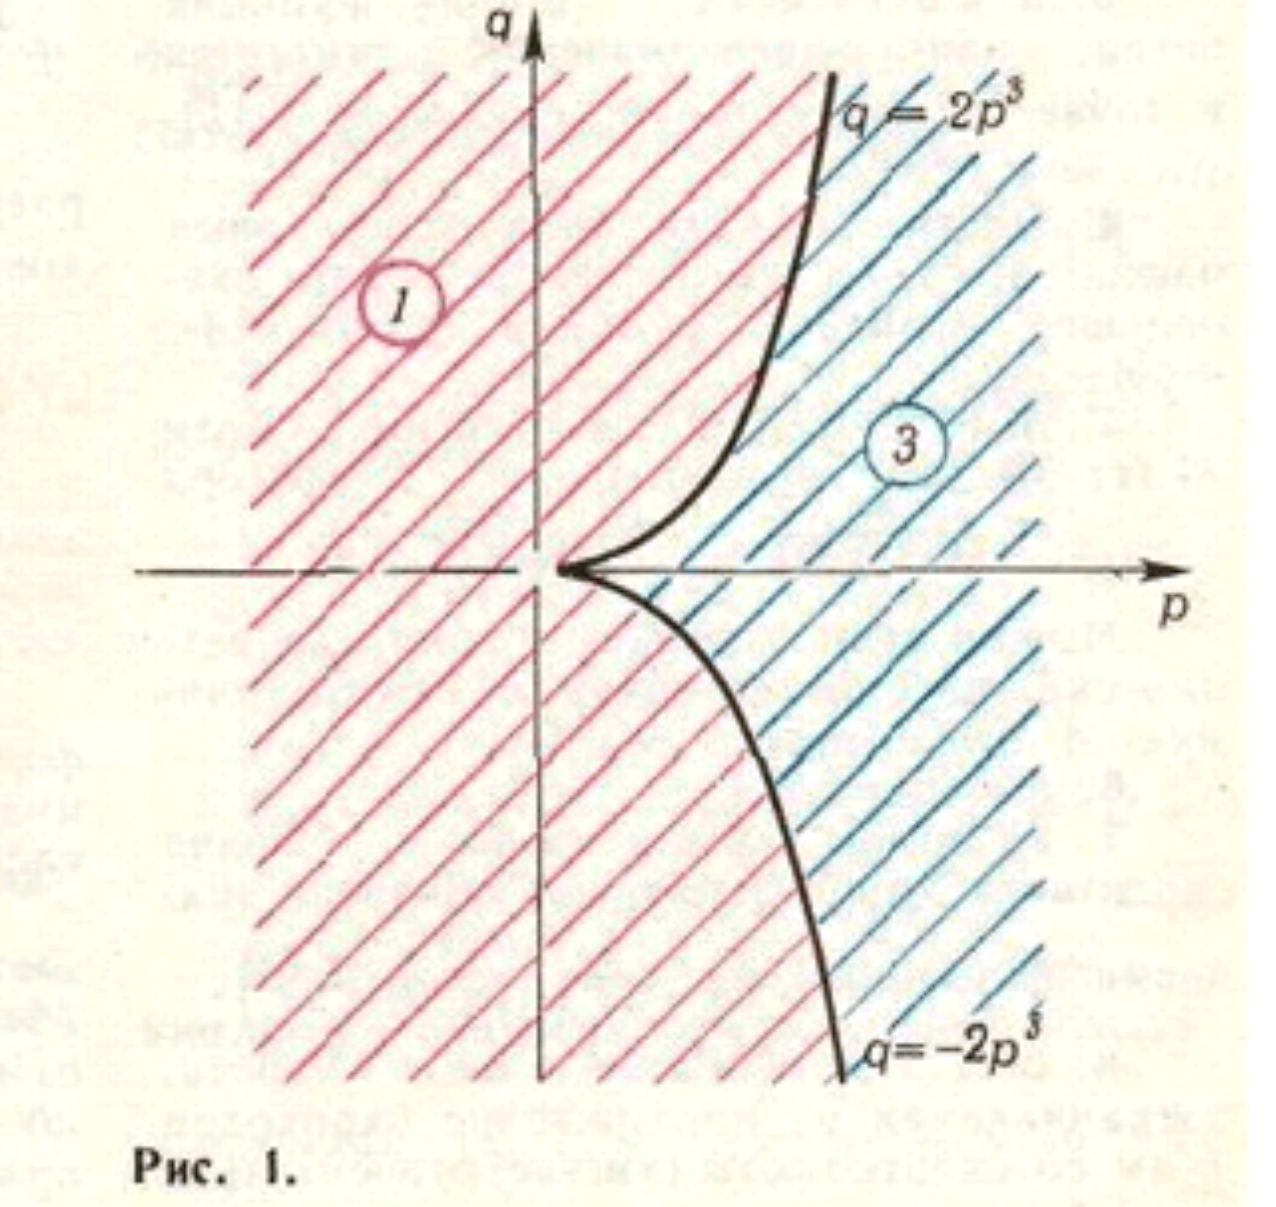
\includegraphics[scale=0.25]{./graph.jpg}
\end{minipage}
\end{document}